% !TEX root = ../main.tex
\begin{figure}[t]
\vspace{-0.5in}
\centering
\iflatexml
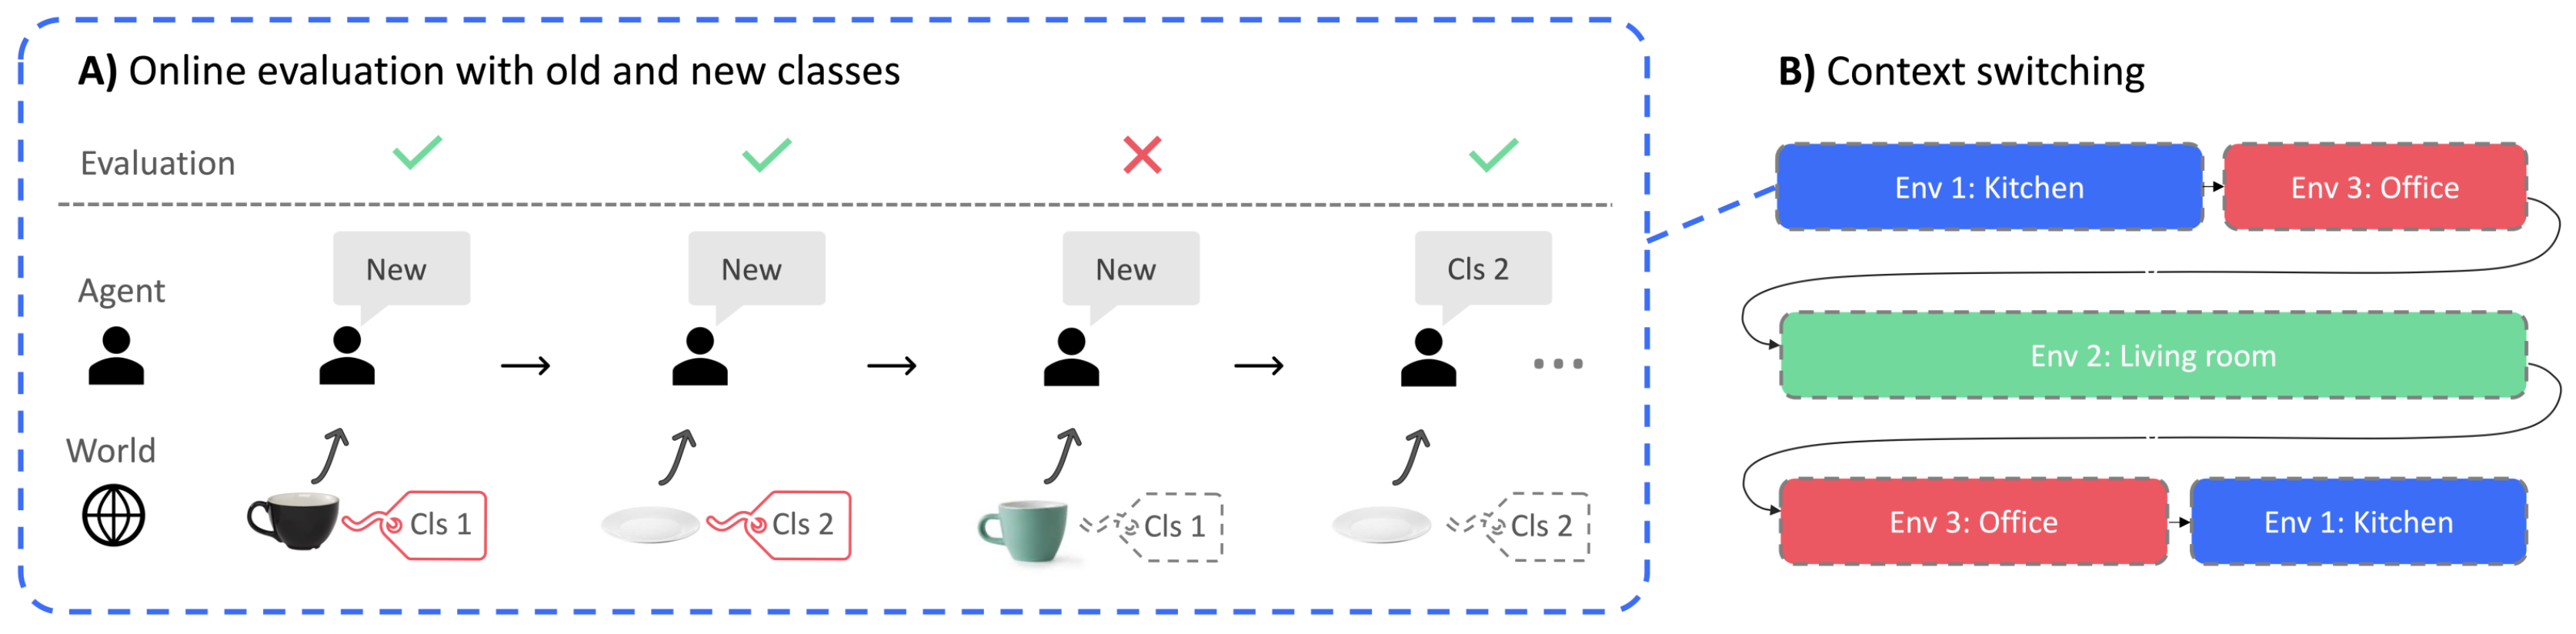
\includegraphics[width=6\textwidth,trim={0.0cm 7.5cm 1.0cm 0},clip]{figures/online_evaluation.png}
\else
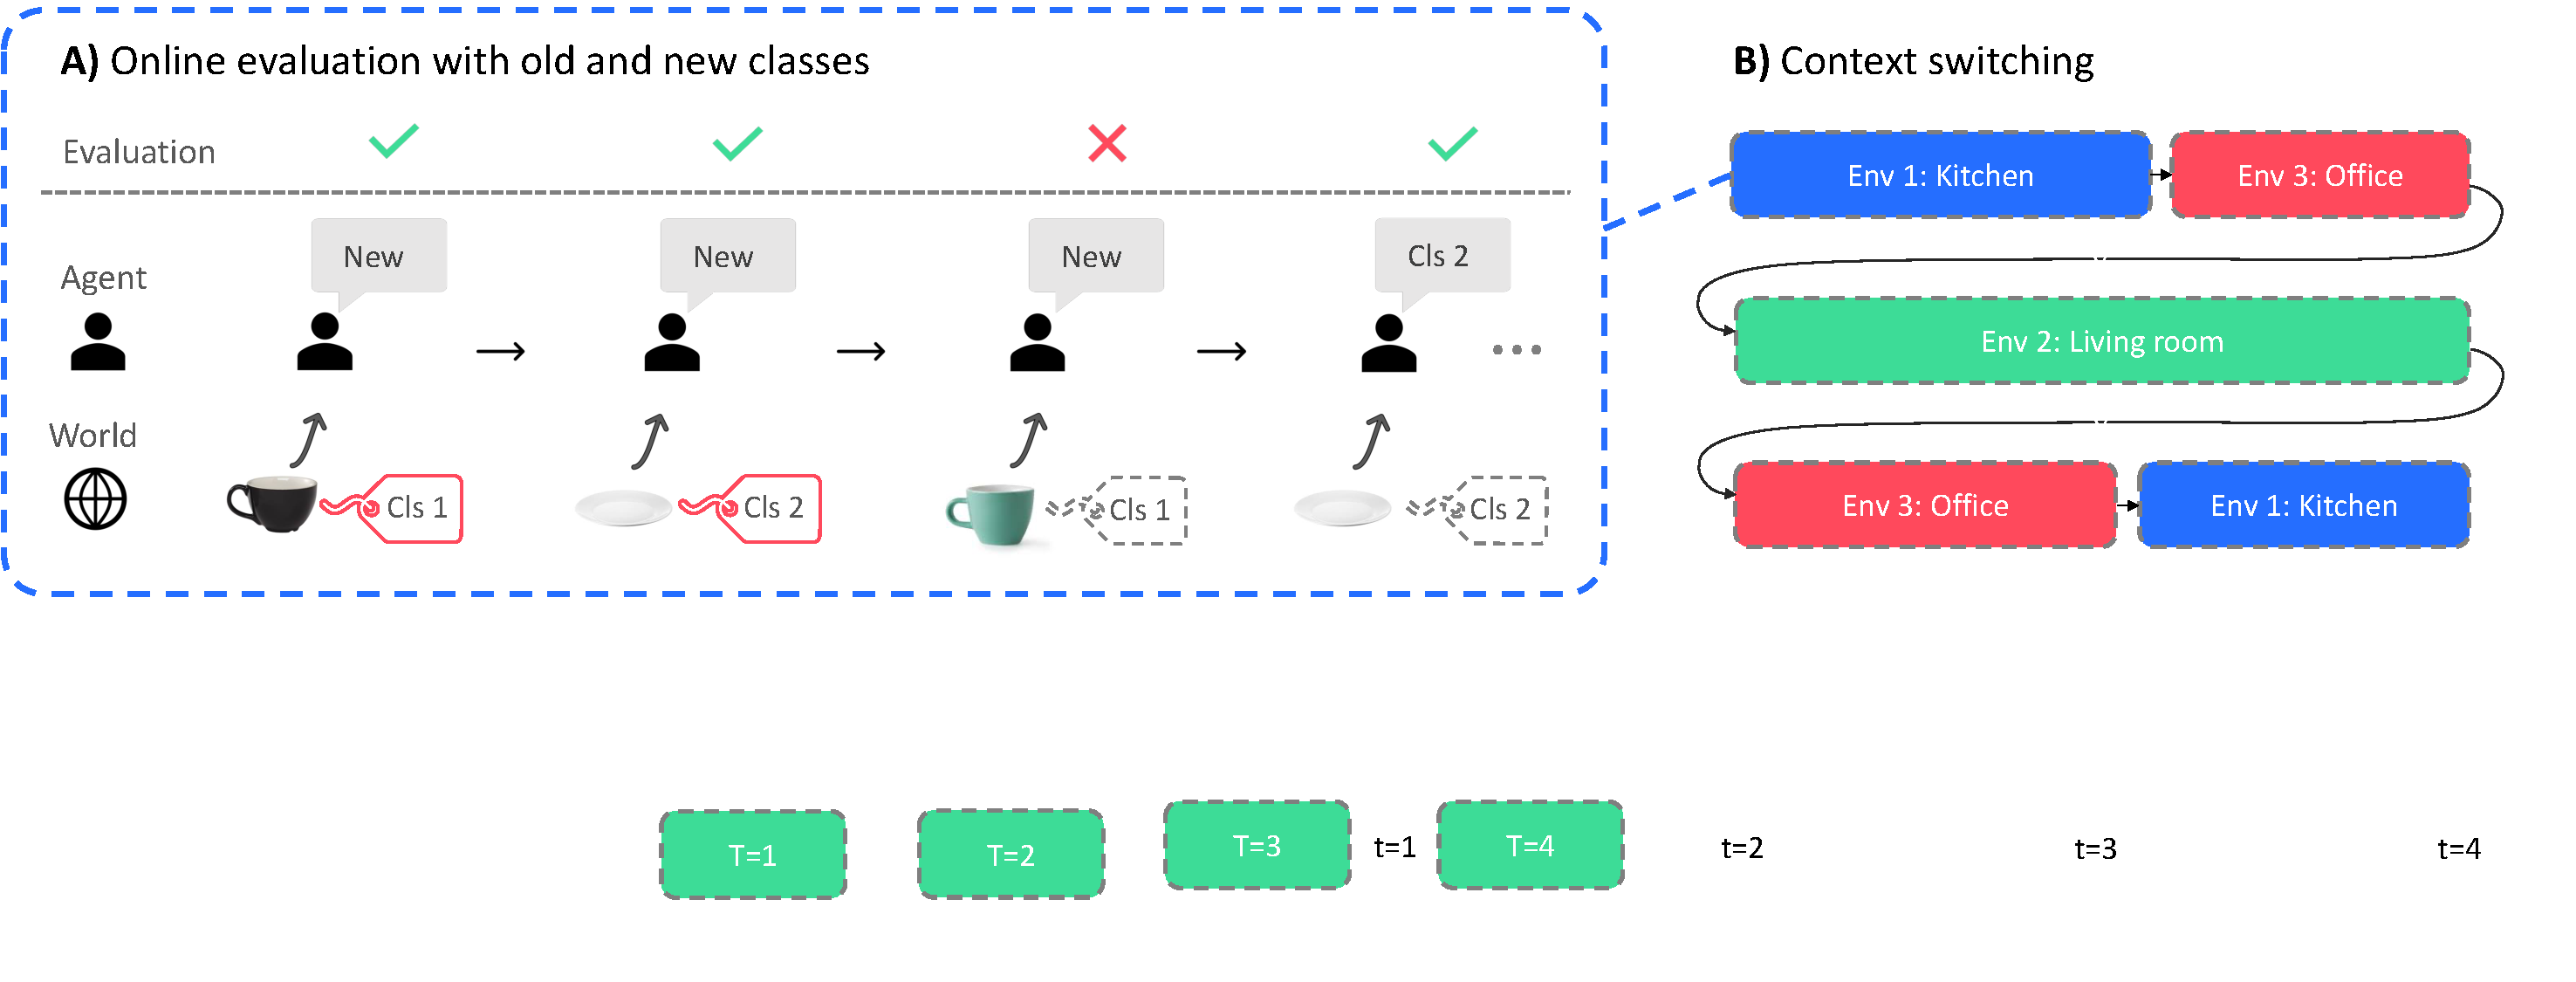
\includegraphics[width=\textwidth,trim={0.0cm 7.5cm 1.0cm 0},clip]{figures/online_evaluation.pdf}
\fi
\vspace{-0.3in}
\caption{\textbf{Online contextualized few-shot learning.} \textbf{A)} Our setup is similar to
online learning, where there is no separate testing phase; model training and evaluation happen
\textit{at the same time}. The input at each time step is an (image, class-label) pair. The number
of classes grows \textit{incrementally} and the agent is expected to answer ``new'' for items that
have not yet been assigned labels. Sequences can be \textit{semi-supervised}; here the label is not
revealed for every input item (labeled/unlabeled shown by red solid/grey dotted boxes). The agent is
evaluated on the correctness of all answers. The model obtains learning signals only on labeled
instances, and is correct if it predicts the label of previously-seen classes, or `new' for new
ones. \textbf{B)} The overall sequence switches between different \textit{learning environments}.
While the environment ID is \textit{hidden} from the agent, inferring the current environment can
help solve the task. }
\label{fig:setup}
\vspace{-0.15in}
\end{figure}
